% !TEX root=../main.tex
\section{Proof of Theorem \ref{thm:rca-l2}}\label{sec:proof-rca-l2}

We define \textit{identifiable intervention recognition} (IIR) as follows:

\begin{definition}[Identifiable Intervention Recognition, IIR]\label{def:identifiable-intervention-recognition}
    % Based on $\mathcal{L}_{1}$ and $P_{\mathbf{m}}$
	Identifiable intervention recognition is to find out a set of potential interventions $\{\mathbf{m}^{\prime} \mid \mathcal{L}_{1}(\mathbf{V} \mid do(\mathbf{m}^{\prime})) \equiv P_{\mathbf{m}} \}$ (\textit{i.e.}, \textit{identifiable interventions}).
\end{definition}

With Definition~\ref{def:identifiable-intervention-recognition}, we have Lemma~\ref{lemma:l2-to-rca} and Lemma~\ref{lemma:rca-to-l2}.

\begin{lemma}\label{lemma:l2-to-rca}
	The knowledge of IIR can be derived from $\mathcal{L}_{2}$.
\end{lemma}
\begin{proof}[Proof of Lemma~\ref{lemma:l2-to-rca}]
	Denote $\mathcal{C}$ as the equivalence classes defined by $\mathcal{L}_{2}$ among $\mathcal{F} = \bigcup_{\mathbf{M} \in 2^{\mathbf{V}}} Val(\mathbf{M})$, where $\mathcal{F}$ is all possible interventions, including no intervention.
	For each equivalent class $c \in \mathcal{C}$, $c$ is a set of interventions $[\mathbf{m}]$ which leads to the same distribution over $\mathbf{V}$:
	$$[\mathbf{m}] = \{\mathbf{m}^{\prime} \mid \mathcal{L}_{1}(\mathbf{V} \mid do(\mathbf{m}^{\prime})) \equiv P_{\mathbf{m}}\}$$
	Denote the distribution of V under $[\mathbf{m}]$ as $\mathcal{L}_{2}^{-1}(P_{\mathbf{m}}) = [\mathbf{m}]$.
	Denote $\mathcal{L}_{2}^{\prime}([\mathbf{m}]) = P_{\mathbf{m}}$, where $[\mathbf{m}] \in \mathcal{C}$.
	For any $\mathbf{m}_{1}, \mathbf{m}_{2} \in \mathcal{F}$, we always have:
	$$P_{\mathbf{m}_{1}} \equiv P_{\mathbf{m}_{2}} \rightarrow [\mathbf{m}_{1}] = [\mathbf{m}_{2}]$$
	Hence, $\mathcal{L}_{2}^{\prime}$ is a one-to-one correspondence and have its inverse mapping, denoted as $\mathcal{L}_{2}^{-1}(P_{\mathbf{m}}) = [\mathbf{m}]$.

	When an intervention occurs, based on $P_{\mathbf{m}} \in \mathcal{L}_{2}(\mathcal{F})$, $\mathcal{L}_{2}^{-1}(P_{\mathbf{m}})$ is the set of targets of IIR.
	Hence, the knowledge of IIR can be derived from $\mathcal{L}_{2}$.
\end{proof}

\begin{lemma}\label{lemma:rca-to-l2}
	The knowledge of IIR encodes $\mathcal{L}_{2}$.
\end{lemma}
\begin{proof}[Proof of Lemma~\ref{lemma:rca-to-l2}]
	For any valid $P_{\mathbf{m}} \in \mathcal{L}_{2}(\mathcal{F})$, IIR will produce a set of possible interventions $\{\mathbf{m}^{\prime} \mid \mathcal{L}_{2}(\mathbf{m}^{\prime}) \equiv P_{\mathbf{m}}\}$.
% 	Notice that the corresponding assignment $\mathbf{m}^{\prime}$ for each possible root cause is just encoded in $P_{\mathbf{m}^{\prime}}$.
	Hence, the knowledge of IIR can be extended to the mapping $\mathcal{L}_{2}^{-1}$ that maps $P_{\mathbf{m}}$ to the element of $\mathcal{C}$.
	Meanwhile, $\mathcal{L}_{2}^{-1}$ is the inverse mapping of $\mathcal{L}_{2}^{\prime}$ and $\mathcal{L}_{2}$ can be derived from $\mathcal{L}_{2}^{\prime}$.
	Hence, the knowledge of IIR encodes $\mathcal{L}_{2}$.
\end{proof}

Based on Lemma~\ref{lemma:l2-to-rca} and Lemma~\ref{lemma:rca-to-l2}, the knowledge of IIR is equivalent to $\mathcal{L}_{2}$.
Then we have \thmref{thm:irca-l2}.

\begin{theorem}\label{thm:irca-l2}
	The knowledge of IIR is at the second layer of the causal ladder.
\end{theorem}

For an SCM with a CBN, we get Lemma~\ref{lemma:decompose-fault}.

\begin{lemma}\label{lemma:decompose-fault}
	For a given SCM $\mathcal{M}$ with a CBN $\mathcal{G}$, let $\mathbf{Pa}(V_{i})$ be the parents of $V_{i}$ in $\mathcal{G}$.
	$P(V_{i} \mid \mathbf{pa}(V_{i}), do(\mathbf{m}))$ can be reduced to the form defined in \eqnref{eqn:parent-block-fault}.
	\begin{equation}\label{eqn:parent-block-fault}
		P(V_{i} \mid \mathbf{pa}(V_{i}), do(\mathbf{m})) = \left\{\begin{array}{ll}
			P(V_{i} \mid \mathbf{pa}(V_{i}), do(v_{i})), & V_{i} \in \mathbf{M} \\
			P(V_{i} \mid \mathbf{pa}(V_{i})), & V_{i} \notin \mathbf{M} \\
		\end{array}\right.
	\end{equation}
\end{lemma}
\begin{proof}[Proof of Lemma~\ref{lemma:decompose-fault}]
	Given a variable $V_{i}$, the intervened variables $\mathbf{M}$ can be separated into three parts: 1) $\mathbf{M}_{Pa} = \mathbf{M} \cap \mathbf{Pa}(V_{i})$, 2) $\mathbf{M}_{i} = \mathbf{M} \cap \{V_{i}\}$, and 3) $\mathbf{M}_{Other} = \mathbf{M} \setminus \mathbf{Pa}(V_{i}) \setminus \{V_{i}\}$.
	Hence, 
	\begin{itemize}
		\item $\mathbf{M} = \mathbf{M}_{Pa} \cup \mathbf{M}_{i} \cup \mathbf{M}_{Other}$,
		\item $\mathbf{M}_{Pa} \cap \mathbf{M}_{i} =  \mathbf{M}_{Pa} \cap \mathbf{M}_{Other} = \mathbf{M}_{i}\cap \mathbf{M}_{Other} = \emptyset$, and
		\item there is no arrow from $\mathbf{M}_{Other}$ to $V_{i}$ in $\mathcal{G}$.
	\end{itemize}

    \paragraph{Case 1.}
    With $V_{i} \in \mathbf{M}$, denote the interventional SCM of $\mathcal{M}$ with $do(\mathbf{m})$ as $\mathcal{M}^{\prime}$.
    $\mathcal{M}^{\prime}$ replaces $f_{i}$ in $\mathcal{M}$ with $v_{i} \gets m_{i}$~\cite{Pearl:2009}.
    As a result, other variables cannot affect  $V_{i}$ any longer.
    Hence, $do(v_{i})$ makes $P(V_{i} \mid \mathbf{pa}(V_{i}), do(\mathbf{m}))$ and $P(V_{i} \mid \mathbf{pa}(V_{i}), do(v_{i}))$ equivalent by $$P(V_{i} \mid \mathbf{pa}(V_{i}), do(\mathbf{m})) = P(V_{i} \mid do(v_{i})) = P(V_{i} \mid \mathbf{pa}(V_{i}), do(v_{i}))$$

    \paragraph{Case 2.}
    With $V_{i} \notin \mathbf{M}$, we get $\mathbf{M}_{i} = \emptyset$ and $\mathbf{M} = \mathbf{M}_{Pa} \cup \mathbf{M}_{Other}$ for the equation below
    $$P(V_{i} \mid \mathbf{pa}(V_{i}), do(\mathbf{m})) = P(V_{i} \mid \mathbf{pa}(V_{i}), do(\mathbf{m}_{Pa}), do(\mathbf{m}_{Other}))$$
    Since $\mathcal{G}$ is a CBN, the ``Parents do/see'' condition~\cite{Bareinboim:2022} states that we can replace $\mathbf{pa}(V_{i})$ with $do(\mathbf{pa}(V_{i}))$.
	\begin{equation}
		P(V_{i} \mid \mathbf{pa}(V_{i}), do(\mathbf{m})) = P(V_{i} \mid do(\mathbf{pa}(V_{i})), do(\mathbf{m}_{Other}))
	\end{equation}
	As we already take $do(\mathbf{m}_{Pa})$ as the condition, the ``Missing-link'' condition~\cite{Bareinboim:2022} ensures that we can drop $do(\mathbf{m}_{Other})$.
	\begin{equation}
		P(V_{i} \mid \mathbf{pa}(V_{i}), do(\mathbf{m})) = P(V_{i} \mid do(\mathbf{pa}(V_{i})))
	\end{equation}
	With the ``Parents do/see'' condition~\cite{Bareinboim:2022} again,  we obtain
	\begin{equation}
		P(V_{i} \mid \mathbf{pa}(V_{i}), do(\mathbf{m})) = P(V_{i} \mid \mathbf{pa}(V_{i}))
	\end{equation}

% 	\begin{enumerate}[label=Case. \arabic*]
% 		\item With $V_{i} \in \mathbf{M}$, denote the interventional SCM of $\mathcal{M}$ with $do(\mathbf{m})$ as $\mathcal{M}^{\prime}$.
% 		$\mathcal{M}^{\prime}$ replaces $f_{i}$ in $\mathcal{M}$ with $v_{i} \gets m_{i}$~\cite{Pearl:2009}.
% 		As a result, other variables cannot affect  $V_{i}$ any longer.
% 		Hence, $do(v_{i})$ makes $P(V_{i} \mid \mathbf{pa}(V_{i}), do(\mathbf{m}))$ and $P(V_{i} \mid \mathbf{pa}(V_{i}), do(v_{i}))$ equivalent by $$P(V_{i} \mid \mathbf{pa}(V_{i}), do(\mathbf{m})) = P(V_{i} \mid do(v_{i})) = P(V_{i} \mid \mathbf{pa}(V_{i}), do(v_{i}))$$

% 		\item With $V_{i} \notin \mathbf{M}$, we get $\mathbf{M}_{i} = \emptyset$ and $\mathbf{M} = \mathbf{M}_{Pa} \cup \mathbf{M}_{Other}$ for the equation below
% 		$$P(V_{i} \mid \mathbf{pa}(V_{i}), do(\mathbf{m})) = P(V_{i} \mid \mathbf{pa}(V_{i}), do(\mathbf{m}_{Pa}), do(\mathbf{m}_{Other}))$$

% 		Since $\mathcal{G}$ is a CBN, the ``Parents do/see'' condition~\cite{Bareinboim:2022} states that we can replace $\mathbf{pa}(V_{i})$ with $do(\mathbf{pa}(V_{i}))$.
% 		\begin{equation}
% 			P(V_{i} \mid \mathbf{pa}(V_{i}), do(\mathbf{m})) = P(V_{i} \mid do(\mathbf{pa}(V_{i})), do(\mathbf{m}_{Other}))
% 		\end{equation}
	
% 		As we already take $do(\mathbf{m}_{Pa})$ as the condition, the ``Missing-link'' condition~\cite{Bareinboim:2022} ensures that we can drop $do(\mathbf{m}_{Other})$.
% 		\begin{equation}
% 			P(V_{i} \mid \mathbf{pa}(V_{i}), do(\mathbf{m})) = P(V_{i} \mid do(\mathbf{pa}(V_{i})))
% 		\end{equation}

% 		With the ``Parents do/see'' condition~\cite{Bareinboim:2022} again,  we obtain
% 		\begin{equation}
% 			P(V_{i} \mid \mathbf{pa}(V_{i}), do(\mathbf{m})) = P(V_{i} \mid \mathbf{pa}(V_{i}))
% 		\end{equation}
% 	\end{enumerate}

	Combining the two cases above provides the final conclusion.
\end{proof}

\begin{proof}[Proof of \thmref{thm:rca-l2}]
	Given an intervention $\mathbf{m}$ and any identifiable intervention $\mathbf{m}^{\prime}$ provided by IIR, $P(\mathbf{V} \mid do(\mathbf{m})) \equiv P(\mathbf{V} \mid do(\mathbf{m}^{\prime}))$.
	Hence, $P(V_{i} \mid \mathbf{pa}(V_{i}), do(\mathbf{m})) \equiv P(V_{i} \mid \mathbf{pa}(V_{i}), do(\mathbf{m}^{\prime}))$ for any $V_{i} \in \mathbf{V}$.
	Notice that the corresponding assignment for an intervention is just encoded in the interventional distribution.
	As a result, $(\forall x \in \mathbf{m}, x^{\prime} \in \mathbf{m}^{\prime}) X=X^{\prime} \rightarrow x=x^{\prime}$.
% 	Notice that the corresponding assignment $\mathbf{m}^{\prime}$ for each possible root cause is just encoded in $P_{\mathbf{m}^{\prime}}$.

	Assume that $\mathbf{m}$ is different from $\mathbf{m}^{\prime}$, \textit{e.g.}, $(\exists X \in \mathbf{V}) X \in \mathbf{M} \wedge X \notin \mathbf{M}^{\prime}$.
	With Lemma~\ref{lemma:decompose-fault}, we have $P(X \mid \mathbf{pa}(X), do(x)) \equiv P(X \mid \mathbf{pa}(X))$, which violates the Faithfulness assumption.
	It is the same for the case $(\exists X \in \mathbf{V}) X \notin \mathbf{M} \wedge X \in \mathbf{M}^{\prime}$.
	Hence, IIR can distinguish $\mathbf{m}$ from other interventions, providing the same answer as IR.

	According to \thmref{thm:irca-l2}, we reach the conclusion that the knowledge of IR is at the second layer of the causal ladder.
\end{proof}

\section{Proof of Theorem \ref{thm:rc-criterion}}\label{sec:proof-rc-criterion}

\begin{proof}[Proof of \thmref{thm:rc-criterion}]
	Notice that $P_{\mathbf{m}}(V_{i} \mid \mathbf{pa}(V_{i})) = P(V_{i} \mid \mathbf{pa}(V_{i}), do(\mathbf{m}))$, while $\mathcal{L}_{1}(V_{i} \mid \mathbf{pa}(V_{i})) = P(V_{i} \mid \mathbf{pa}(V_{i}))$.

    \paragraph{Case 1.}
    With $V_{i} \in \mathbf{M}$, we get $\mathbf{M}_{i} = \{V_{i}\}$.
	Under the Faithfulness assumption, \eqnref{eqn:faithfulness-conditional} must hold, while Lemma~\ref{lemma:decompose-fault} provides $P(V_{i} \mid \mathbf{pa}(V_{i}), do(\mathbf{m})) = P(V_{i} \mid \mathbf{pa}(V_{i}), do(v_{i}))$.
	\begin{equation}\label{eqn:faithfulness-conditional}
		P(V_{i} \mid \mathbf{pa}(V_{i}), do(v_{i})) \neq P(V_{i} \mid \mathbf{pa}(V_{i}))
	\end{equation}
	Hence, $$V_{i} \in \mathbf{M} \Rightarrow P_{\mathbf{m}}(V_{i} \mid \mathbf{pa}(V_{i})) \neq \mathcal{L}_{1}(V_{i} \mid \mathbf{pa}(V_{i}))$$
	
	\paragraph{Case 2.}
	With $V_{i} \notin \mathbf{M}$, Lemma~\ref{lemma:decompose-fault} provides $P(V_{i} \mid \mathbf{pa}(V_{i}), do(\mathbf{m})) = P(V_{i} \mid \mathbf{pa}(V_{i}))$.
	Hence, $$V_{i} \notin \mathbf{M} \Rightarrow P_{\mathbf{m}}(V_{i} \mid \mathbf{pa}(V_{i})) = \mathcal{L}_{1}(V_{i} \mid \mathbf{pa}(V_{i}))$$
	Its contrapositive stands as well, $$P_{\mathbf{m}}(V_{i} \mid \mathbf{pa}(V_{i})) \neq \mathcal{L}_{1}(V_{i} \mid \mathbf{pa}(V_{i})) \Rightarrow V_{i} \in \mathbf{M}$$, which is the converse proposition of Case 1.

% 	\begin{enumerate}[label=Case. \arabic*]
% 		\item With $V_{i} \in \mathbf{M}$, we get $\mathbf{M}_{i} = \{V_{i}\}$.
% 		Under the Faithfulness assumption, \eqnref{eqn:faithfulness-conditional} must hold, while Lemma~\ref{lemma:decompose-fault} provides $P(V_{i} \mid \mathbf{pa}(V_{i}), do(\mathbf{m})) = P(V_{i} \mid \mathbf{pa}(V_{i}), do(v_{i}))$.
% 		\begin{equation}\label{eqn:faithfulness-conditional}
% 			P(V_{i} \mid \mathbf{pa}(V_{i}), do(v_{i})) \neq P(V_{i} \mid \mathbf{pa}(V_{i}))
% 		\end{equation}
% 		Hence, $$V_{i} \in \mathbf{M} \Rightarrow P_{\mathbf{m}}(V_{i} \mid \mathbf{pa}(V_{i})) \neq \mathcal{L}_{1}(V_{i} \mid \mathbf{pa}(V_{i}))$$

% 		\item With $V_{i} \notin \mathbf{M}$, Lemma~\ref{lemma:decompose-fault} provides $P(V_{i} \mid \mathbf{pa}(V_{i}), do(\mathbf{m})) = P(V_{i} \mid \mathbf{pa}(V_{i}))$.
% 		Hence, $$V_{i} \notin \mathbf{M} \Rightarrow P_{\mathbf{m}}(V_{i} \mid \mathbf{pa}(V_{i})) = \mathcal{L}_{1}(V_{i} \mid \mathbf{pa}(V_{i}))$$
% 		Its contrapositive stands as well, $$P_{\mathbf{m}}(V_{i} \mid \mathbf{pa}(V_{i})) \neq \mathcal{L}_{1}(V_{i} \mid \mathbf{pa}(V_{i})) \Rightarrow V_{i} \in \mathbf{M}$$, which is the converse proposition of Case 1.
% 	\end{enumerate}

    In conclusion, $V_{i} \in \mathbf{M} \Leftrightarrow P_{\mathbf{m}}(V_{i} \mid \mathbf{pa}(V_{i})) \neq \mathcal{L}_{1}(V_{i} \mid \mathbf{pa}(V_{i}))$.
% 	Combine the two cases above, and we reach the conclusion
% 	$$V_{i} \in \mathbf{M} \Leftrightarrow P_{\mathbf{m}}(V_{i} \mid \mathbf{pa}(V_{i})) \neq \mathcal{L}_{1}(V_{i} \mid \mathbf{pa}(V_{i}))$$
\end{proof}

\section{Implementation Details}\label{sec:implementation-details}

\subsection{Baseline Methods}

Most of the code in this work is written in Python, while we adopt the R package pcalg~\cite{Kalisch:2012} for the PC algorithm.
We utilize process-based parallel programming to isolate errors only.

NSigma calculates $\max_{t} \frac{\lvert v_{i}^{(t)} - \mu_{i} \rvert}{\sigma_{i}}$.
We adopt the authors' implementation\footnote{https://github.com/Amossys-team/SPOT} for SPOT~\cite{Siffer:2017} while re-implementing ENMF~\cite{Cheng:2016} in Python based on the authors' MATLAB implementation\footnote{https://github.com/chengw07/CausalRanking}.
The other baseline methods are not publicly available.
We implement them by our understanding.

\subsection{Simulation Data Generation}

We generate the simulation datasets based on the Vector Auto-regression model, as shown in \eqnref{eqn:var}.
Following existing work~\cite{Zheng:2018,He:2021}, the value of non-zero elements in the weighted adjacent matrix, $A_{ij}$, is uniformly sampled from $(-2.0, -0.5) \cup (0.5, 2.0)$.
For the second item $\beta \mathbf{x}^{(t-1)}$, we set $\beta = 0.1$ in the experiment.
Finally, we sample the standard deviations from an exponential distribution for the zero-mean Gaussian noises $\mathbf{\epsilon}^{(t)}$.

The structure of $A$ is generated in two steps, as shown in \algref{alg:sedag-generation}.
We first generate a tree to ensure that the graph is a connected DAG.
Then, the other edges are inserted randomly.

\begin{algorithm}[htb]
	\caption{Graph Generation in the Simulation Study}\label{alg:sedag-generation}
	\begin{algorithmic}[1]
		\REQUIRE $N_{node}$, the number of nodes; $N_{edge}$, the number of edges
		\STATE $\mathcal{G} \gets (\mathbf{V}, \mathbf{E})$, where $\mathbf{V} = \{1, 2, \cdots, N_{node}\}$
		\FOR{$i = 2, \cdots, N_{node}$}
		    \STATE $j \gets$ choose one node from $\{1, 2, \cdots, i - 1\}$ randomly
		    \STATE Add the edge $i \rightarrow j$ into $\mathbf{E}$
		\ENDFOR
		\FOR{$k = N_{node}, N_{node} + 1, \cdots, N_{edge}$}
		    \STATE $i, j \gets$ sample $i, j \in \mathbf{V}$ randomly, \textit{s.t.}, $i > j \wedge (i \rightarrow j) \notin \mathbf{E}$
		    \STATE Add the edge $i \rightarrow j$ into $\mathbf{E}$
		\ENDFOR
		\RETURN $\mathcal{G}$
	\end{algorithmic}
\end{algorithm}

\subsection{Structural Graph Construction}

In the empirical study, we construct the structural graph for the Oracle database instances.
\figref{fig:oracle-architecture} shows the SQL processing and memory structures in the call graph.
\figref{fig:performance:case} further shows part of the graph among metrics.
We drop metrics not included in the final structural graph, as our knowledge fails to cover them.
Baseline methods only use labeled metrics for a fair comparison.

\begin{figure}[htb]
	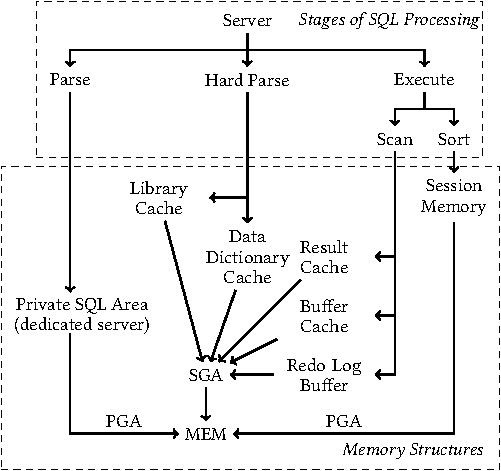
\includegraphics{img/oracle-architecture}
	\caption{Part of the Oracle database call graph}\label{fig:oracle-architecture}
	\Description{
    	This figure shows the Stages of SQL Processing and Memory Structures.
    	We convert the related documentation into such a call graph.
	}
\end{figure}

\subsection{Regression Method Selection}\label{sec:regression-method-selection}

\tableref{tab:performance:oracle:regression} shows RHT's performance with several regression methods.
RHT with the linear regression (\textit{Linear}) has unsatisfying performance, as the relations among real-world variables are seldom linear.
Support Vector Regression (\textit{SVR}) with the sigmoid kernel, which is non-linear, improves the performance.
\citeauthor{Fu:2021} provide a way to predict distribution based on Random Forest (RF) and Mixture Density Networks (MDN), respectively, instead of a single value~\cite{Fu:2021}.
Hence, RHT combined with RF or MDN can measure the deviation for a new datum against the predicted distribution.
However, these two methods perform worse than the simple linear regression due to a limited understanding of the normal status, as shown in \figref{fig:ood}.
As a result, we choose SVR in the empirical study.

\begin{table}[tb]
	\caption{RHT with different regression methods on $\mathcal{D}_{O}$}\label{tab:performance:oracle:regression}
	\begin{tabular}{lrrrrr}
		\toprule
		\multirow{2}{0.18\columnwidth}{Regression Method} & \multirow{2}{*}{AC@1} & \multirow{2}{*}{AC@3} & \multirow{2}{*}{AC@5} & \multirow{2}{*}{Avg@5} & \multirow{2}{0.08\columnwidth}{T (s)} \\
		& & & & & \\
		\midrule
        Linear & 0.197 & 0.424 & 0.556 & 0.409 & 0.559 \\
        SVR & \textbf{0.328} & \textbf{0.601} & \textbf{0.677} & \textbf{0.546} & 0.834 \\
        RF & 0.202 & 0.394 & 0.525 & 0.382 & 22.065 \\
        MDN & 0.111 & 0.212 & 0.253 & 0.195 & 694.329 \\
		\bottomrule
	\end{tabular}
\end{table}
